\documentclass{report}
\usepackage[utf8]{inputenc}

\usepackage{algorithm}
\usepackage{algorithmicx} % Doc is at http://tug.ctan.org/macros/latex/contrib/algorithmicx/algorithmicx.pdf
\usepackage{algpseudocode}
\usepackage{amsfonts} % for R symbol (the set of real numbers)
\usepackage{color}
\usepackage{colortbl} % for \rowcolor
\usepackage[pdftex]{graphicx}
\usepackage{graphicx}
\usepackage[bookmarks=false]{hyperref}
\hypersetup{colorlinks=true,linkcolor=black,citecolor=black,filecolor=black,urlcolor=blue}
\usepackage{mathtools}
\usepackage{multirow}
\usepackage{stmaryrd} % for llbracket and rrbracket
\usepackage{subcaption}
\usepackage{nicefrac}
\usepackage{amsmath}
\usepackage{amssymb}
\usepackage{stmaryrd}
\usepackage{amsthm}
\usepackage{wrapfig}
\usepackage{multicol}
\usepackage{flushend}

\usepackage[bookmarks=false]{hyperref}\hypersetup{colorlinks=true,linkcolor=black,citecolor=black,filecolor=black,urlcolor=blue}


\usepackage{verbatim}
\usepackage{hyperref}

\newcommand{\tristan}[1]{\color{red}{TG: #1}\color{black}}
\title{Stream summarization for connected objects}
\author{BO LI }

\usepackage{natbib}
\usepackage{graphicx}
\graphicspath{ {images/} }

%\tableofcontents

\begin{document}

\maketitle

\chapter{Introduction}

%IoT, Embedded system, sensors,
%Motsai(internship coding), Neblina, Big Data, Stream

\begin{comment}
context
problem description
goal motivation
outline and contribution(publication)
sensor network 技术将会引来更多的挑战,随着无线连通的普及,the units in IoT will reach 26 billion by 2020(Gartnar 2014)
IoT越来越普及,因为智能家居的普及,我们的生活就围绕IoT中。再这个网络中objects 可以互相交流。很多家居都拥有嵌入式系统,从而可以通过终端e.g.手机,电脑进行控制,比如用手机操作灯的开 关,空调温度的高低...同时多样的传感器时生活更加智能,aceleramiter....
给我们生活提供更加有效的信息。同时当big data, 数据分析兴起的时候,数据变得尤为重要,越来越有价值,但是因为sensor 产生的都是stream data, 它带来了一些挑战。
1,2,3
(数据流无法再次查询,需要空间存储数据,但是devices空间是由限制的,尽管)
因此再数据流信息的挖掘中,有很多之前的研究。
。。。。
。。。
。。。。
然而再现实世界中,sensor 网络中的devices没有过多的空间 severs KB, 并且电量是有限的。因此在sensor网络中,如果我们要传输大量的数据,电量会消耗很多。数据需要发发送到client端,不管是通过 Wifi, Bluetooth etc. 
\end{comment}

With the recent technological advances internet of Things(IoT) applications, the connected devices In IoT will reach 75 billion by 2025\footnote{\url{ https://www.statista.com/statistics/471264/iot-number-of-connected-devices-worldwide}}. In industrial domains, the connected objects are often used for capturing properties such as temperature, and receiving signal or data from others. In domestic domains, many household products are expected to provide more function which could make live more convenient and improve the quality of life. For example, aggregating embedded system with air conditions and light in order to simply control them with our smart electronics e.g. Mobile phone and PC. The most typical network of connected object is WSNs, which are being increasingly deployed for enabling continuous monitoring and sensoring of physical variables of our world~\cite{li2016temporal}.

And with the rise of data science, the data become more and more important cause it could provide knowledges and informations after filter and learning.
Thus The stream data produced in IoT also improtant. But cause the characteristic of stream data, it it needed to process stream data timely due to its volume and velocitym. We may lose the opportunity to process them at all, if we did not do it in real time. So some previous research has discussed various stream analytic problems, such as estimating cardinality, frequency moments and clustering.

Power consumption is among the biggest challenges targeting connected 
objects, particularly in the industrial domains, where several sensing 
systems are commonly launched in the field to run for days or even 
weeks without being recharged. Typically, such devices use sensors to 
capture properties such as temperature or motion, and stream them to a 
host system over a radio transmission protocol such as Bluetooth 
Low-Energy (BLE). System designers aim to reduce the rate of data 
transmission as much as possible, as radio transmission is a 
power-hungry operation.

Compression is a key technique to reduce the rate of radio 
transmission.  While in several applications lossless compression 
methods are more desirable than lossy compression techniques, in the 
context of IoT and sensor data streams, the measured sensor data 
intrinsically involves noise and measurement errors, which can 
be treated as a configurable tolerance for a lossy compression algorithm. 

Resource-intensive lossy compression algorithms such as the ones based on 
polynomial interpolation, discrete cosine and Fourier transforms, or 
auto-regression methods~\cite{lu2010optimized} are not well-suited for 
connected objects, due to the limited memory available on 
these systems (typically a few KB), and the energy consumption 
associated with CPU usage. Instead, compression algorithms need 
to find a trade-off between reducing network communications and 
increasing memory and CPU usage. As 
discussed in~\cite{zordan2014performance}, linear compression methods 
provide a very good compromise between these two factors, leading to 
substantial energy reduction.

% lossy vs lossless compression

% LTC summary
% define transmitted, received points, copmression ratio
The Lightweight Temporal Compression method 
(LTC~\cite{schoellhammer2004lightweight}) has been designed 
specifically for energy-constrained systems, initially sensor networks. 
It approximates data points by a piece-wise linear function that 
guarantees an upper bound on the reconstruction error, and a reduced 
memory footprint in $\mathcal{O}(1)$. However, LTC has only been 
described for 1D streams, while streams acquired by connected objects, such as 
acceleration or gyroscopic data, are often multi-dimensional. 

In this paper, we extend LTC to dimension $n$. To do so, we propose an 
algebraic formulation of the algorithm that also yields a 
norm-independent expression of it. We implement our extension on 
Motsai's Neblina module\footnote{\url{ https://motsai.com/products/neblina}}, and we test it on 3D acceleration streams 
acquired during human exercises, namely biceps curling, walking and 
running. Our implementation of LTC is available as free software.

We assume that the stream consists of a sequence of data points 
received at uneven intervals. The compression algorithm 
\emph{transmits} fewer points than it receives. The transmitted points 
might be included in the stream, or computed from stream points. The 
\emph{compression ratio} is the ratio between the number of received 
points and the number of transmitted points. An application 
reconstructs the stream from the transmitted points: the 
\emph{reconstruction error} is the maximum absolute difference between 
a point of the reconstructed stream, and the corresponding 
point in the original stream.

\setlength{\textfloatsep}{0pt}
\begin{figure}[b]
\centering
\includegraphics[width=\columnwidth]{./figures/ltc.pdf}
\caption{Illustration of the LTC algorithm. Blue 
dots are received points, red dots are transmitted points. Dashed lines 
represent the high and low lines when a point is 
transmitted.\vspace*{-0.3cm}}
\label{fig:ltc}
\end{figure}

% Outline
Section~\ref{sec:ltc} provides some background on the LTC algorithm, 
and formalizes the description initially proposed 
in~\cite{schoellhammer2004lightweight}. Section~\ref{sec:extension} 
presents our norm-independent extension to dimension $n$, and 
Section~\ref{sec:implementation} describes our implementation. 
Section~\ref{sec:results} reports on experiments to validate our 
implementation, and evaluates the impact of n-dimensional LTC on 
energy consumption of connected objects.

\chapter{Related Work}
\section{Stream}


\section{Compression}
\subsection{LEC}
LEC
Marcelloni, Francesco, and Massimo Vecchio. "A simple algorithm for data compression in wireless sensor networks." IEEE communications letters 12.6 (2008): 411-413.

local data compression has been classified into two main techniques in~\cite{srisooksai2012practical}: lossless compression algorithm, which do not lose information during compression and depression process and lossy compression algorithm, which may lose some information.
In lossless compression algorithm, there are two type of algorithm: one is based on dictionary approach, another one is based on predictive coding approaches~\cite{srisooksai2012practical}.
\subsection{Dictionary based lossless compression algorithm}
\subsection{A simple lossless entropy compression (LEC) scheme}
LEC algorithm is first proposed in ~\cite{marcelloni2008simple} which is a approximated version of exponential-Golomb code~\cite{teuhola1978compression}.
In paper~\cite{marcelloni2008simple}, authors measured temperature and humidity by sensors and compressed data by using LEC.It uses very small dictionary whose size is determined by the number of the bits after ADC converter~\cite{marcelloni2008simple}. 
For instance, in a sensor node, a measure $m_i$ is gained and converted into numeral value $r_i$ represented on R bit by ADC. At each new data point $r_i$, LEC compute the difference of adjacent points $d_i$ = $r_i$ - $r_{i-1}$, in order to compute $d_0$, the $r_-1$ equals the central value among $2^R$. The difference $d_i$ Encoded by entroy encoder, and represented as a bit sequence in 2 parts $s_i | a_i$ , where $s_i$ is the number of the bits needed to represent the difference $d_i$, and $a_i$ represent $d_i$ based on special rule.In the paper~\cite{marcelloni2008simple}, the authors generated the $s_i$ by Huffman coding. Let's say the $n_i$ is the Decimal expression of $s_i$,then $n_i = \lceil\log{_2}{\left|{b_i}\right|}\rceil$~\cite{marcelloni2008simple} and $n_i \leq R$. Then $s_i$ could be generated by searching Huffman code with $n_i$. Table 1 is used in paper~\cite{marcelloni2008simple}. From the table, it support R+1 symbol($s_i$) and each symbol $s_i$ contains $2^{n_i}$ numeral value. The $a_i$ part would be generated as follow:

$a_i$ is null, when $d_i$ = 0, $s_i$ = 0
$a_i$ = $2^{n_i} - 1 + d_i$ when $d_i < 0$
$a_i$ = $d_i$ when $d_i > 0 $



%At first, for any measure mi is transformed by analog-to-digital converter into a binary representation ri on R bits~\cite{marcelloni2008simple}. The value differences $d_i = r_i - r_{i-1}$. assuming $r_{-1}$ equal control value among possible value in order to compute $d_0$.  Then Representing each $d_i$ with $s_i|a_i$, $s_i$ is computed according to $n_i$ where $n_i = \lceil\log_2(\abs{d_i})\rceil$ which is not bigger than R,$s_i$ is a variable-length binary string generated from $n_i$ by using Huffman code. For $a_i$ part in $s_i|a_i$, when $d_i>0$, $a_i$ is  $n_i$ low-order bits of two’s complement of $d_i$. $d_i<0$ , $a_i$ is $n_i$ low-order bits of the two’s complement of $(d_i - 1)$. When $d_i =0$, $s_i$ is 00 and $a_i$ is not presented.~\cite{marcelloni2008simple}

In order to operating this algorithm, it’s necessary to save the table in to memory. when a new data $r_i$ come, we need to compute the $d_i$ at first, and then represent the $d_i$ to $s_i|a_i$ with searching table. For the table it only needs small constants memory space.

%Due to limited resourses in IoT devices, the power saving is need to extend the work life of devices. LEC is a lossless comprssion method, In the paper~cite{marcelloni2008simple}, the authors generated the $s_$ by Huffman coding. Let's say the$n_i$ is the Decimal expression of $s_i$, then $n_i$ = \lceil \log_2^(\mid d_i \mid) \rceil$
\subsection{S-LEC}
dictionary 
S-LZW which is a algorithm adopts and modifies the well know lossless algorithm LZW


1. LZW
2. S-LZW


traditional predictive coding 

1. TMT
2. LEC
3. ALFC

Piecewise linear approximation

1. LTC
2. PLAMLiS and its variant

emerging technique 

1. compression sensing


both lossless and lossy


for GPC framework
1. TMT  entropy coding (lossless)
    |-->  entropy coding  ->  alphabet or symbol table
        |--> 0M-based alphabet system
2. Lossy compression
    |--> synchronized iterative multistep predictoin
    cause errors propagate and accumlate sample
        |--> BLC block lossy compression

\subsection{LTC}
\label{sec:ltc}
LTC approximates the data stream
by a piece-wise linear function of time, with an error bounded by parameter $\epsilon$.

\subsubsection{Notations}

The algorithm receives a stream of data points $x_i$
at times $t_i$ ($i \in \mathbb{N}$), and it transmits a stream of data points $\xi_i$
at times $\tau_i$ ($i \in \mathbb{N}$). To simplify the notations, we assume that:
\begin{equation*}
\forall k \in \mathbb{N}, \  \exists ! i \in \mathbb{N} \  \tau_k = t_i
\end{equation*}
That is, transmission times coincide with reception times.
We define the \emph{shifted received points} as follows:
\begin{equation*}
\forall k \in \mathbb{N}\ , \forall j \in \mathbb{N^*},\ (u^k_j, y^k_j) = (t_{i+j}, x_{i+j}), 
\end{equation*}
where $i$ is such that $t_i = \tau_k$ and:
\begin{equation*}
\forall k \in \mathbb{N},\  (u^k_0, y^k_0) = (\tau_k, \xi_k).
\end{equation*}
This definition is such that $y^k_j$ is the $j^{th}$ data point received
after the $k^{th}$ transmission and $u^k_j$ is the corresponding timestamp.
Figure~\ref{fig:ltc} illustrates the notations and algorithm.

The LTC algorithm maintains two lines, the \emph{high line}, and the
\emph{low line} defined by (1) the latest transmitted point and (2) the
\emph{high point} (high line) and the \emph{low point} (low line). When
a point ($t_i$, $x_i$) is received, the high line is updated as
follows: if $x_i+\epsilon$ is below the high line then the high line is
updated to the line defined by the last transmitted point and ($t_i$,
$x_i+\epsilon$); otherwise, the high line is not updated. Likewise, the low line
is updated from $x_i-\epsilon$. Therefore, any line located between the
high line and the low line approximates the data points received since
the last transmitted point with an error bounded by $\epsilon$.

\begin{algorithm}
\begin{algorithmic}[1]
\Input
   \Desc{$(u^k_j, y^k_j)$}{$\quad \quad $Received data stream}\newline
   \Desc{$\epsilon$}{$\quad \quad$Error bound}\newline
\EndInput
\Output
   \Desc{tr}{Transmitted points}\newline
\EndOutput
\State tr = $(u^0_0, y^0_0)$ \Comment{Last transmitted point}
\State k = 0 ; j = 1
\State (lp, hp) = ($y^0_1 - \epsilon$, $y^0_1 + \epsilon$) \Comment{Low and high points}

\While{True} \Comment{Process received points as they come}
    \State j += 1
    \State new\_lp = max($y^k_j-\epsilon$, line($u^k_j$, tr, ($u^k_{j-1}$, lp)))
    \State new\_hp = min($y^k_j+\epsilon$, line($u^k_j$, tr, ($u^k_{j-1}$, hp)))
    \If{new\_lp $\leq$ new\_hp} \Comment{Keep compressing}
        \State (lp, hp) = (new\_lp, new\_hp)
    \Else
        \State tr = $(u^k_{j-1}, (lp+hp)/2)$
        \Comment{Transmit point}
        \State k += 1
        \State j = 1
        \State (lp, hp) = ($y^k_j-\epsilon$, $y^k_j+\epsilon$)
    \EndIf
\EndWhile
\end{algorithmic}
\caption{Original LTC algorithm, adapted from~\cite{schoellhammer2004lightweight}.}
\label{algo:ltc}
\end{algorithm}

Using these notations, the original LTC algorithm can
be written as in Algorithm~\ref{algo:ltc}. For readability, we assume
that access to data points is blocking, i.e., the program will wait
until the points are available. We also assume that the content of
variable \texttt{tr} is transmitted after each assignment of this
variable. Function \texttt{line}, omitted for brevity, returns the
ordinate at abscissa $x$ (1st argument) of the line defined by the points
in its 2nd and 3rd arguments.

\subsection{Regression}


\chapter{Extension of LTC to n Dimension}
In this section we provide a norm-independent formulation of LTC in
dimension $n$. By $n$ we refer to the dimension of the data points
$x_i$. To handle time, LTC actually operates in dimension
$n+1$.

\subsection{Preliminary comments}

We note that the formulation of LTC 
in~\cite{schoellhammer2004lightweight} relies on the intersection of 
\emph{convex cones} in dimension $n+1$. For $n=1$, it corresponds to 
the intersection of triangles, which can efficiently be computed by 
maintaining boundary lines, as detailed previously. In higher 
dimension, however, cone intersections are not so straightforward, due 
to the fact that the intersection between cones may not be a cone.

To address this issue, we formulate LTC as an intersection test between
\emph{balls} of dimension $n$, that is, segments for $n=1$, disks for
$n=2$, etc. Balls are defined from the \emph{norm} used in
the vector space of data points. For $n=1$, the choice of the norm does
not really matter, as all p-norms and the infinity norm are identical.
In dimension $n$, however, norm selection will be critical.

\subsection{Algebraic formulation of LTC}

\subsubsection{Definitions}

Let $(u_0^k, y_0^k) \in \mathbb{R}^{n+1}$ be the latest transmitted point. For convenience, all the subsequent points will be
expressed in the orthogonal space with origin $(\tau_k, \xi_k)$. We denote by $(v_j, z_j)_{j \in \llbracket 0, m \rrbracket}$ such points:
\begin{equation*}
\forall j \leq m,\  (v_j, z_j) = (u_j^k - \tau_k, y_j^k - \xi_k)
\end{equation*}
Let $\mathcal{B}_j$ be the ball of $\mathbb{R}^n$ of centre $\frac{v_1}{v_j}z_j$ and radius
$\frac{v_1}{v_j}\epsilon$:
\begin{equation*}
\mathcal{B}_j = \left\{ z \in \mathbb{R}^n,\\norm{z-\frac{v_1}{v_j}z_j} \leq\frac{v_1}{v_j}\epsilon \right\}
\end{equation*}
Note that $v_1$ is defined as soon as one point is received after the last
transmission.

\subsubsection{LTC property}

We define the \emph{LTC property} as follows:
\begin{equation*}
\exists z \in \mathbb{R}^n, \ \forall j \in \llbracket 1, m \rrbracket, \norm{\frac{v_j}{v_1}z-z_j} \leq \epsilon.
\end{equation*}
The original LTC algorithm ensures that the LTC property is
verified between each transmission. Indeed, all the data points
$z$ such that $(v_1, z)$ is between the high line and the low line
verify the property. Line 13 in Algorithm~\ref{algo:ltc} guarantees that
such a point exists.

The LTC property can be re-written as follows:
\begin{equation*}
\exists z \in \mathbb{R}^n, \ \forall j \in \llbracket 1, m \rrbracket, \norm{z-\frac{v_1}{v_j}z_j} \leq \frac{v_1}{v_j}\epsilon
\end{equation*}
that is:
\begin{equation}
\bigcap_{j=1}^m \mathcal{B}_j \neq \O
\label{eq:ltc-property}
\end{equation}
Note that $(\mathcal{B}_j)_{j \in \llbracket 1, m \rrbracket}$ is a sequence
of balls of strictly decreasing radius, since $v_j > v_1$.

\subsection{Algorithm}

The LTC algorithm generalized to dimension $n$ tests that the LTC 
property in Equation~\ref{eq:ltc-property} is verified after each reception of a data 
point. It is written in Algorithm~\ref{algo:general-ltc}.
\begin{algorithm}
\begin{algorithmic}[1]
\Input
   \Desc{$(u^k_j, y^k_j)$}{$\quad \quad $Received data stream}
   \Desc{$\epsilon$}{$\quad \quad$Error bound}
\EndInput
\Output
   \Desc{tr}{Transmitted points}
\EndOutput

\State tr = ($\tau, \xi$) = ($u^0_0, y^0_0$) \Comment{Last transmitted point}
\State k = 0 ; j = 0
\While{True}
    \State j += 1
    \State ($v_j, z_j$) = ($u_j^k - \tau, y_j^k - \xi$)
    \If{$\bigcap_{l=1}^j{\mathcal{B}_l} = \O$}
        \State Pick $z$ in $\bigcap_{l=1}^{j-1}{\mathcal{B}_j}$ \Comment{Transmit point}
        \State tr = ($\tau$, $\xi$) = ($u^k_{j-1}, z$)
        \State k += 1
        \State j = 1
    \EndIf
\EndWhile
\end{algorithmic}
\caption{Generalized LTC.}
\label{algo:general-ltc}
\end{algorithm}

\subsection{Ball intersections}

Although Algorithm~\ref{algo:general-ltc} looks simple, one should not
overlook the fact that there is no good general algorithm to test
whether a set of balls intersect. The best general algorithm we could find
so far relies on Helly's theorem which is formulated as follows~\cite{helly1923mengen}:
\begin{theorem}
Let $\left\{ X_i \right\}_{i \in \llbracket 1, m \rrbracket}$ be a collection of convex subsets of $\mathbb{R}^n$. If the intersection of every $n+1$
subsets is non-empty, then the whole collection has an non-empty intersection.
\end{theorem}
\noindent This theorem leads to an algorithm of complexity ${m \choose n+1}$ which is
not usable in resource-constrained environments.

The only feasible algorithm that we found is norm-specific. It
maintains a representation of the intersection
$\bigcap_{j=1}^{m}{\mathcal{B}_j}$ which is updated at every iteration.
The intersection tests can then be done in constant time. However,
updating the representation of the intersection may be costly
depending on the norm used. For the infinity norm, the representation
is a rectangular cuboid which is straightforward to update by
intersection with an n-ball.
For the Euclidean norm, the representation is a volume with no particular property,
which is more costly to maintain.

\subsection{Effect of the norm}

As mentioned before, norm selection in $\mathbb{R}^n$ has a critical
impact on the compression error and ratio. To appreciate this effect,
let us compare the infinity norm and the
Euclidean norm in dimension 2. By comparing the unit disk to a
square of side 2, we obtain that the compression ratio of a random stream would
be $\frac{4}{\pi}$ times larger with the infinity norm than with the 
Euclidean norm. In 3D, this ratio would be $\frac{6}{\pi}$. Conversely, 
a compression error bounded by $\epsilon$ with the infinity norm 
corresponds to a compression error of $\frac{\epsilon}{\sqrt{n}}$ with 
the Euclidean norm. Unsurprisingly, the
infinity norm is more tolerant than the Euclidean norm.

It should also be noted that using the infinity norm in $\mathbb{R}^n$ 
boils down to the use of the 1D LTC algorithm independently in each 
dimension, since a data point will be transmitted as soon as the linear 
approximation doesn't hold in any of the dimensions. For the Euclidean 
norm, however, the multidimensional and multiple unidimensional 
versions are different: the multiple unidimensional version 
behaves as the infinity norm, but the multidimensional version is more 
stringent, leading to a reduced compression rate and error.

To choose between the multidimensional implementation and multiple 
unidimensional ones, we recommend to check whether the desired 
error bound is expressed independently for every sensor, or as an aggregate error between them.
The multidimensional version is
more appropriate for multidimensional sensors, for instance 3D 
accelerometers or 3D gyroscopes, and the multiple unidimensional 
version is more suitable for multiple independent sensors, for 
instance a temperature and a pressure sensor.
%~ For instance, in case of a 3D accelerometer, if the error 
%~ is expressed simply as 
%~ ``10~mg", then the multidimensional version should be chosen because it 
%~ will guarantee that the norm of the 3D acceleration vector will be 
%~ reconstructed with an error less than 10~mg. Conversely, if the error is 
%~ specified as ``10~mg in x, 
%~ 10~mg in y and 10~mg in z", then the multiple unidimensional version 
%~ should be used.

\chapter{Implementation}
\section{Implement LTC n-dimension}
To implement LTC in nD with the infinity norm, we maintain a cuboid 
representation of $\cap_{l=1}^j{\mathcal{B}_l}$ across the 
iterations of the \texttt{while} loop in 
Algorithm~\ref{algo:general-ltc}. The implementation works with
constant memory and requires limited CPU time.

With the Euclidean norm, the intersection test is more complex. We keep 
in memory a growing set $S$ of balls and the bounding box $B$ of their 
intersection. Then, when a new point arrives, we consider the 
associated ball $\mathcal{B}_j$ and our intersection test works as in 
Algorithm~\ref{algo:euclidean}. \texttt{box} is a function that returns 
the bounding box of an n-ball. \texttt{find\_bisection(S, B)} searches 
for a point in all the elements in S, using plane sweep and bisection 
initialized by the bounds of B. Our code is available at 
\url{https://github.com/big-data-lab-team/stream-summarization} under 
MIT license.


Assume the stream $j_{th}$ data	
$D_i = (x_{j1}, x_{j2}, ..., x_{jn},t_i)$, the first data $D_0$ would	
be save as base point $Z=(z_{1}, z_{2}, ..., z_{n},t_z)$in the Method.	
As usual, produce a n-ball ${\mathcal{B}_j}$ in n-dimension after mapping the data point into mapping plane.
We also need to record the intersect $S$ for finding Bounding Box of the intersection of balls in $S$.
\begin{comment}
The first data $D_1$ would change into tolerance range $R_1$.	
initializing $S = R_1$. For each follow data$ D_i, i>1$, mapping $D_1$	
into $\hat{D_1}$ = $(\{\hat{x_{ij}}=z_j + \frac{x_{ij}-z_{j}}{t_i-t_z} \mid1\leqslant{j}\leqslant{n}\},t_i)$,	
and error margin after mapping should be $\frac{\epsilon}{t_i-t_z}$	
on $\hat{x_{ij}}, j={1...n}$. The tolerance range after R_i, intersect	
with S, if there is overlap, update S = S intersect R_i. If not, the base point	
would be transmitted and select a point in S as base point with timestamp $t_{i-1}$.	
\end{comment}
At beginning of the in function \texttt{find\_bisection(S, B)}, we have a new $S$ which include $\mathcal{B}_j$, and updated Bounding box $\mathcal{B}$. According the $\mathcal{B}$, we could know the new n-ball $\mathcal{B}_j$ has intersect with the cuboid bounding box. Selecting one dimension at first e.g. $x_1$, we can easily know the range of intersection in $x_1$ axis, $x_1.min$ and $x_1.max$ represents the minimum and maximum value in $x_1$ axis respectively. Then using the bisection function find midum value $x_1.mid$ = $\frac{x_1.max + x_1.min}{2}$, and search each n-ball in $S$, to find bounding range in other axis, e.g. $x_2$ by using $x_1 = x_1.mid$. If $x_2.min \leqslant x_2.max$, it means in $x_1 = x_1.mid$ we could find a intersected point in $x_2$ axis, than we need to continue the search, which try to find a overlap in axis $x_3$ with $x_1 = x_1.mid$ and $x_2 = x_2.mid$, and repeat it until finding a intersection in all axis, $x_i.max \geqslant x_i.min$, $i = \{1...n \}$. the $x_2.min > x_2.max$, it means no intersection in $x_1 = x_1.mid$, also it shows that there is not an public intersection in updated $S$. Otherwise,  If the $x2.min \leqslant x2.max$,  it means no intersection in $x1=x1.mid$, we need to continue bisection. During the procession, we would record two n-balls, one has maximum $x_2.min$ and another has minimum $x_2.max$. Computing intersect point $E$ between line of two n-ball's centers and intersecting serface. If $E.x_1$ is larger than x_1.mid, than go ahead bisection with updating x_1.min = x_1.mid. Otherwish, continuing with x_1.max = x_1.mid.

\todo{need descript function find_bisection}



\begin{comment}

At beginning of the algorithm, we need a base point (which we will call \textit{z}) and bounding box which has upper and lower bound for each parameter respectively.Then start the algorithm.	
\begin{enumerate}	
  \item Initialization: Get first data point, and set point \textit{z} equals to first data point. Get the second data point $(x_{21},...,x_{2n},t_2)$, and assign each upper bound $U_j = x_{2j}+\frac{\epsilon}{t_2-t_1}$ and lower bound $L_j = x_{2j}-\frac{\epsilon}{t_2-t_1}$ where $j=\{1...n\}$.	
  \item Get next data point, map the data point $(x_{i1},...,x_{in},t_i)$ into $(\{\hat{x_{ij}}=z_j + \frac{x_{ij}-z_{j}}{t_i-t_z} \mid1\leqslant{j}\leqslant{n}\},t_i)$.	
  \item For each parameter(dimension) \textit{j}, if upper bound $U_j$ smaller than $x_{ij}-\frac{\epsilon}{t_i-t_1}$ or lower bound $L_j$ bigger than $x_{ij}+\frac{\epsilon}{t_i-t_1}$, then \textbf{goto 5}, else $U_j = min(U_j, x_{ij}+\frac{\epsilon}{t_i-t_1})$, and $L_j = max(L_j, x_{ij}-\frac{\epsilon}{t_i-t_1})$.	
  \item Goto 2.	
  \item output \textit{z} data point.	
  \item Reset: set data point \textit{z} equals to center of the bounding box with time-stamp $t_{i-1}$, and $U_j=x_{ij}+\frac{\epsilon}{t_i-t_{i-1}}$, $L_j =x_{ij}-\frac{\epsilon}{t_i-t_{i-1}}$ with $j=\{1...n\}$.	
  \item Goto 2.	
  \item After all, output \textit{z} data point and center of bounding box respectively.	
\end{enumerate}	


 for tolerance range, it depends on EPSILON and different type of distances for EPSILON.	As reference above, the norm selection is importance. In this section,
If we using Manhattan distance to create tolerance range, it would become rectangle in 2D and cube for 3D.	we show the implementation of infinity norm and Euclidean norm.
But the tolerance range wold become disk or ball in 2D and 3D respectively, by using Euclidean distance.
\end{comment}

\begin{algorithm}
\begin{algorithmic}[1]
\Input
   \Desc{$S$}{Set of intersecting balls}
   \Desc{$B$}{Bounding box of the intersection of balls in $S$}
   \Desc{$\mathcal{B}_j$}{New ball to check}
\EndInput
\Output
   \Desc{$S$}{Updated set of intersecting balls}
   \Desc{$B$}{Updated bounding box}
   \Desc{$T$}{True if all the balls in S and $\mathcal{B}_j$ intersect}
\EndOutput

\If{$\mathcal{B}_j \cap B = \O$} \Comment{Ball is outside bounding box}
\State \Return ($S$, $B$, False) 
\EndIf
\If{$\exists\ \mathcal{B}_i \in S$ s.t. $\mathcal{B}_j \cap \mathcal{B}_i = \O$}
\State \Return ($S$, False) \Comment{Some balls don't intersect}
\EndIf
\If{$\exists\ \mathcal{B}_i \in S$ s.t. $\mathcal{B}_j \subset \mathcal{B}_i$} \Comment{Remove inclusions}
\State Remove $\mathcal{B}_i$ from $B$. Add $\mathcal{B}_j$ to $B$.
\EndIf
\State $B$ = box($\mathcal{B}_j$) $\ \bigcap\ $ $B$
\State $S$ = $S \ \bigcup \  \{\mathcal{B}_j\}$
\State $x$ = find\_bisection($S$, $B$) \Comment{This can take some time}
\If{$x$ == Null}
\State \Return ($S$, $B$, False)
\Else
\State \Return ($S$, $B$, True)
\EndIf
\end{algorithmic}
\caption{Intersection test for Euclidean n-balls.}
\label{algo:euclidean}
\end{algorithm}

\begin{comment}
In Euclidean distance version, we also map the coming data into same	
time-stamp $t_1$ the timestamp after base point. The difference with	
Manhattan distance version is that recording overlapping part with	
a post-designed model is difficult, which need retain several arcs in	
2-dimension, or convex surfaces in 3-dimension. In our method, we will	
record all tolerance range for every mapped data which come from base	
data point until coming data point, in order to checking if there is	
intersection among them. For instance, in 3D-t, assume we have a the	
base point $Z = D_0$ and the tolerance range $R_1$ which is a ball	
as the intersection S. we need a list L to record mapped balls	
from $D_1$ to coming data. For each comming data $D_i, i>1$ mapping	
this data into $t_1$, and add it into list. Then the work is check out	
if all balls intersect, and form a public intersection. The method is	
based on plane sweep and binary search. At first, select one parameter,	
such as x-axis, finding a bounding range of all balls $B_i$ in x-axis.	
suppose $Max_bound_x = Min{1..n}{B_i.center.x + EPSILON/i}$, and	
$Min_bound_x = Max{1..n}{B_i.center.x - EPSILON/i}$. If there is overlap	
among balls, then the axis of the points inside intersection must located	
between Min_bound_x and Max_bound_x. Using binary search to select	
mid_x = (Min_bound_x + Max_bound_x)/2, then calculate a y-axis bounding	
with the plane x = mid_x. If the get bounding range in y-axis where	
$Max_bound_y > Min_bound_y$ and using binary search again to find mid_y,	
It means there is a line x=mid_x, Max_bound_y>= y >= Min_bound_y,	
parallels z-axis, could pass through all balls. Finally, in z-axis,	
computing bounding range, and If $Max_bound_z > Min_bound_z$, there	
must be one or more points inside all balls. The problem be solved.	
If the loop of binary search in x-axis overs, then there is no public	
intersection among balls, and need to transmit and update base point.	
In this method we need O(n*logn*logn) time complexity for binary search	
in x-axis and y-axis and traversal all balls in z-axis, also O(n) space	
complexity is needed for maintaining list. According this method,	
it could be extended into N-dimensional data. The main idea is to search,	
dimension by dimension, from a room or plane or line and get intersection	
point finally.
\end{comment}



\begin{algorithm}
    \begin{flushleft}
        \textbf{function} Recursive$(left, right, j, p)$  -- $j$ means $j_th$ dimension
    \end{flushleft}
    \begin{algorithmic}[1]
        \WHILE{$left \leqslant right$}
            \STATE $mid \gets (left + right)/2$
            \STATE $max \gets +\infty$
            \STATE $min \gets -\infty$
            \FOR{$i=1$ \textbf{to} $tmp\_list.length$}
                \STATE $P_1$ and $P_2$ are intersection points of $tmp\_list[i]$ and line $d_{j}=mid$, $(P1.d_{j-1}\geqslant P2.d_{j-1})$
                \IF{$P_1.d_{j-1} < max$}
                    \STATE $max \gets p_1.d_{j-1}$
                    \STATE $max\_index \gets i$
                \ENDIF
                \IF{$P_2.d_{j-1} > min$}
                    \STATE $min \gets p_2.d_{j-1}$
                    \STATE $min\_index \gets i$
                \ENDIF
            \ENDFOR
            \IF{$max >= min$}
                \STATE $p.d_j \gets mid$
                \IF{Recursive$(min, max, j-1, p)$}
                    \STATE \textbf{return} true
                \ENDIF
            \ENDIF
            \STATE Assume $P_d$ is the intersection between common chord of two objects $tmp\_list[max\_index]$, $tmp\_list[min\_index]$ and their line of centers.
            \IF{$P_d.d_j < mid$}
                \STATE $right \gets mid-1$
            \ELSIF{$P_d.d_j > mid$}
                \STATE $left \gets mid+1$
            \ENDIF

         \ENDWHILE
        \RETURN false
    \end{algorithmic}
\end{algorithm}

\section{Implement polynomial regression}

\chapter{Experiments and Results}
\section{LTC with n-dimension with LTC original}
We conducted two experiments using Motsai's Neblina 
module, a system 
with a Nordic Semiconductor nRF52832 micro-controller, 64~KB of RAM, 
and Bluetooth Low Energy connectivity. Neblina has a 3D 
accelerometer, a 3D gyroscope, a 3D magnetometer, and environmental 
sensors for humidity, temperature and pressure. The platform is 
equipped with sensor fusion algorithms for 3D orientation tracking and 
a machine learning engine for complex motion analysis and motion 
pattern recognition~\cite{sarbishei2016accuracy}. Neblina has a 
battery of 100mAh; at 200~Hz, its average consumption is 2.52~mA when using 
accelerometer and gyroscope sensors but without radio 
transmission, and 3.47~mA with radio transmission, leading to an 
autonomy of 39.7~h without transmission and 28.8~h with transmission. 

\subsection{Experiment 1: validation}

%\todo{(Put a picture of Neblina in a box worn 
%on the wrist)}
\begin{wrapfigure}{R}{3cm}
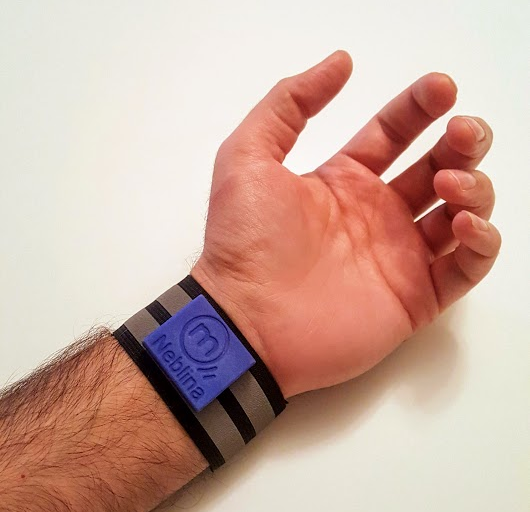
\includegraphics[width=3cm]{figures/neblina-wrist.png}
\caption{Setup with Neblina.}
\label{fig:neblina-wrist}
\end{wrapfigure}
We validated the behaviour of our LTC extension on a PC using data 
acquired with Neblina. We collected two 3D accelerometer time-series, a 
short one and a longer one, acquired on two different subjects 
performing biceps curl, with a 50~Hz sampling rate (see 
Figure~\ref{fig:datasets-1}). In both cases, the subject was wearing 
Neblina on their wrist, as in Figure~\ref{fig:neblina-wrist}. It should be noted that the longest
time-series also has a higher amplitude, perhaps due to differences between 
subjects.

\begin{figure*}
\centering
\begin{subfigure}{1.85\columnwidth}
\centering
\includegraphics[width=0.3\columnwidth]{figures/5-time-bicep-curl-plot-x.pdf}
\includegraphics[width=0.3\columnwidth]{figures/5-time-bicep-curl-plot-y.pdf}
\includegraphics[width=0.3\columnwidth]{figures/5-time-bicep-curl-plot-z.pdf}
\caption{Short biceps curl$^a$}
\end{subfigure}

{\footnotesize $^a$ Average 
of az data is -7.81mg. It was shifted to 0 so that the graphs can all 
use the same y scale.}

\begin{subfigure}{1.85\columnwidth}
\centering
\includegraphics[width=0.3\columnwidth]{figures/Mohammad-bicep-curl-plot-x.pdf}
\includegraphics[width=0.3\columnwidth]{figures/Mohammad-bicep-curl-plot-y.pdf}
\includegraphics[width=0.3\columnwidth]{figures/Mohammad-bicep-curl-plot-z.pdf}
\caption{Long biceps curl}
\end{subfigure}

\caption{Time-series used in Experiment 1}
\label{fig:datasets-1}
\end{figure*}

We compressed the time-series with various values of $\epsilon$, using 
our 2D (x and y) and 3D (x, y and z) implementations of LTC. On 
Neblina, the raw uncalibrated accelerometer data corresponds to errors 
around 20~mg (1~g is 9.8~m/s$^2$). We used a 
laptop computer with 16~GB of RAM, an Intel i5-3210M CPU @ 2.50GHz 
$\times$ 4, and Linux Fedora 27. We measured memory consumption using 
Valgrind's massif 
tool~\cite{nethercote2006building}, 
and processing time using \texttt{gettimeofday()} from the GNU C 
Library. 

Results are reported in Table~\ref{table:results-validation}. 
As expected, the compression ratio increases with $\epsilon$, and the 
maximum measured error remains lower than $\epsilon$ in all cases. The 
maximum is reached most of the time on these time-series.

\paragraph{Infinity vs Euclidean norms}
The average ratio between the compression ratios obtained
with the infinity and Euclidean norm is 1.03 for 2D data, and 1.06
for 3D data. These ratios are lower than the theoretical values of
$\frac{4}{\pi}$ in 2D and $\frac{6}{\pi}$ in 3D, which are obtained for
random-uniform signals. Unsurprisingly, the infinity norm surpasses the
Euclidean norm in terms of resource consumption. Memory-wise, the
infinity norm requires a constant amount of 80~B, used to store the
intersection of n-balls. The Euclidean norm, however, uses up to 4.7~KB of memory
for the Long time-series in 3D with $\epsilon$=48.8~mg. More importantly,
the amount of required memory increases for longer time-series, and it also increases with larger
values of $\epsilon$. Similar observations are made for the processing
time, with values ranging from 0.4~ms for the simplest time-series and
smallest $\epsilon$, to 41.3~ms for the most complex time-series and
largest~$\epsilon$.
%~ Figure~\ref{fig:memory} shows the memory consumption
%~ of the 3D Euclidean implementation for $\epsilon$=48.8~mg: peaks appear
%~ at the end of long compressed ranges where the signal was $\epsilon$-closed
%~ to the linear approximation.

\paragraph{2D vs 3D}
For a given $\epsilon$, the compression
ratios are always higher in 2D than in 3D. It makes sense since the
probability for the signal to deviate from a straight line
approximation is higher in 3D than it is in 2D. Besides, resource
consumption is higher in 3D than in 2D: for the infinity norm, 3D
consumes 1.4 times more memory than 2D (1.8 times on average for
Euclidean norm), and processing time is 1.35 longer (1.34 on
average for Euclidean norm).

\begin{table}
    \begin{subfigure}{\columnwidth}
    \centering
    \begin{tabular}{l|l|l|l|l}
    \hline
    \rowcolor{headcolor}
                           & \multicolumn{2}{c|}{Infinity} & \multicolumn{2}{c}{Euclidean}\\
    \rowcolor{headcolor}
    $\epsilon$  (mg)          & 48.8         & 34.5       & 48.8       & 34.5 \\
    \hline
    Max error   (mg)          & 48.8         & 34.4       & 48.8       & 34.5 \\
    Compression ratio (\%)    & 79.77        & 72.59      & 77.49      & 70.96\\
    Peak memory   (B)         & 80           & 80         & 688        & 688  \\
    Processing time (ms)      & 0.101        & 0.094      & 0.456      & 0.406\\ \hline
    \end{tabular}
    \caption{Short biceps curl (2D)}
    \end{subfigure}\\
    \begin{subfigure}{\columnwidth}
    \centering
    \begin{tabular}{l|l|l|l|l}
    \hline
    \rowcolor{headcolor}
                   & \multicolumn{2}{c|}{Infinity} & \multicolumn{2}{c}{Euclidean} \\
    \rowcolor{headcolor}
    $\epsilon$ (mg)            & 48.8        & 34.5       & 48.8        & 34.5    \\
    \hline
    Max error  (mg)            & 48.8        & 34.5       & 48.8        & 34.5             \\
    Compression ratio (\%)     & 77.46       & 70.98      & 75.77       & 68.81           \\
    Peak memory  (B)           & 80          & 80         & 2512        & 2608             \\
    Processing time (ms)       & 6.06        & 5.84       & 33.84       & 31.07           \\ \hline
    \end{tabular}
    \caption{Long biceps curl (2D)}
    \end{subfigure}\\
    \begin{subfigure}{\columnwidth}
    \centering
    \begin{tabular}{l|l|l|l|l}
    \hline
    \rowcolor{headcolor}
                           & \multicolumn{2}{c|}{Infinity} & \multicolumn{2}{c}{Euclidean} \\
    \rowcolor{headcolor}
    $\epsilon$ (mg)        & 48.8          & 28.2          & 48.8   & 28.2   \\
    \hline
    Max error  (mg)        & 48.8          & 28.2          & 48.8   & 28.2   \\
    Compression ratio (\%) & 78.14         & 66.39         & 74.39  & 63.13   \\
    Peak memory (B)        & 112           & 112           & 1744   & 784    \\
    Processing time (ms)   & 0.147         & 0.134         & 0.731  & 0.514  \\ \hline
    \end{tabular}
    \caption{Short biceps curl (3D)}
    \end{subfigure}\\
    \begin{subfigure}{\columnwidth}
    \centering
    \begin{tabular}{l|l|l|l|l}
    \hline
    \rowcolor{headcolor}
                              & \multicolumn{2}{c|}{Infinity} & \multicolumn{2}{c}{Euclidean} \\
    \rowcolor{headcolor}
    $\epsilon$ (mg)                & 48.8        & 28.2       & 48.8     & 28.2    \\
    \hline
    Max error  (mg)                & 48.8        & 28.2       & 48.8     & 28.2    \\
    Compression ratio (\%)         & 71.23       & 58.11      & 67.35    & 53.24   \\
    Peak memory (B)                & 112         & 112        & 4752     & 3856    \\
    Processing time (ms)           & 7.87        & 7.22       & 41.29    & 39.04   \\ \hline
    \end{tabular}
    \caption{Long biceps curl (3D)}
    \end{subfigure}
    \caption{Results from Experiment 1}
    \label{table:results-validation}
\end{table}

\begin{figure*}
\centering
\begin{subfigure}{1.85\columnwidth}
\centering
\includegraphics[width=0.3\columnwidth]{./figures/walking-1000-x.pdf}
\includegraphics[width=0.3\columnwidth]{./figures/walking-1000-y.pdf}
\includegraphics[width=0.3\columnwidth]{./figures/walking-1000-z.pdf}
\caption{Walking}
\end{subfigure}
\begin{subfigure}{1.85\columnwidth}
\centering
\includegraphics[width=0.3\columnwidth]{./figures/running-1000-x.pdf}
\includegraphics[width=0.3\columnwidth]{./figures/running-1000-y.pdf}
\includegraphics[width=0.3\columnwidth]{./figures/running-1000-z.pdf}
\caption{Running}
\end{subfigure}
\caption{Time series used in Experiment 2 \vspace*{-0.3cm}}
\label{fig:datasets-2}
\end{figure*}

%~ \begin{figure}
%~ \includegraphics[width=\columnwidth]{./figures/memory-mohammad.pdf}
%~ \caption{Memory usage of 3D Euclidean implementation, long biceps curl time-series, $\epsilon$=48.8~mg.}
%~ \label{fig:memory}
%~ \end{figure}

\subsection{Experiment 2: impact on energy consumption}

We acquired two 3D accelerometer time-series at 200~Hz for two 
activities: walking and running (see Figure~\ref{fig:datasets-2}). In 
both cases, the subject was wearing Neblina on their wrist as in 
Experiment 1. We collected 1,000 data points for each activity, 
corresponding to 5 seconds of activity.

We measured energy consumption associated with the transmission of 
these time-series by ``replaying" the time-series after loading them as 
a byte array in Neblina. We measured the current every 500~ms. We also 
measured the max and average latency resulting from compression.

 Results are reported in Table~\ref{table:results-energy}. For a given
 $\epsilon$ and norm, the compression ratio is larger for walking than
 for running. The ratio of saved energy is relative to the reference
 current of 3.47~mA measured when Neblina transmits data without
 compression. In all cases, activating compression saves energy. The 
 reduction in energy consumption behaves as the compression ratio: it 
 increases with $\epsilon$, it is higher for the infinity norm than for 
 the Euclidean, and it is higher for the walking activity than for 
 running. For a realistic error of $\epsilon$=9.8~mg, the ratio of 
 saved energy with the infinity norm is close to 20\% for the walking 
 activity, which is substantial. Latency is higher for walking 
 than for running, and it is also higher for the Euclidean norm than 
 for the infinity norm. In all cases, the latency remains lower 
 than the 5-ms tolerable latency at 200~Hz, which demonstrates the 
 feasibility of 3D LTC compression.

\begin{table}[]
   \begin{subfigure}{\columnwidth}
   \centering
   \begin{tabular}{l|l|l|l|l|l|l}
   \hline
   \rowcolor{headcolor}
                          & \multicolumn{3}{c|}{Infinity} & \multicolumn{3}{c}{Euclidean} \\
   \rowcolor{headcolor}
   $\epsilon$ (mg)             & 48.8    & 9.8      & 4.9   & 48.8   & 9.8   & 4.9   \\
   \hline
   Max error (mg)              & 48.8    & 9.8      & 4.9   & 48.8   & 9.8   & 4.9   \\
   Compr.      ratio (\%)      & 88.9    & 66.4     & 45.5  & 87.6   & 63.3  & 37.2  \\
   Average (mA)                & 2.64    & 2.79     & 3.02  & 3.10   & 3.02  & 3.13  \\
   Saved energy (\%)           & 23.9    & 19.7     & 13.0  &  10.7  & 13.0  & 9.7   \\
   Max latency ($\mu$s)& 60      & --       & --    & 1530   & --    & --    \\
   Average latency ($\mu$s) & 31 & --       & --    & 145    & --    & --    \\    
   \hline
   \end{tabular}
   \caption{Walking}
   \end{subfigure}
   \begin{subfigure}{\columnwidth}
   \centering
   \begin{tabular}{l|l|l|l|l|l|l}
   \hline
   \rowcolor{headcolor}

                     & \multicolumn{3}{c|}{Infinity} & \multicolumn{3}{c}{Euclidean} \\
    \rowcolor{headcolor}
   $\epsilon$ (mg)        & 48.8       & 9.8      & 4.9       & 48.8      & 9.8    & 4.9    \\
   \hline
   Max error (mg)         & 48.8       & 9.8      & 4.9       & 48.8      & 9.8    & 4.9   \\
   Compr.      ratio (\%) & 68.6       & 25.5     & 9.5       & 64.4      & 19.8   & 5.7   \\
   Average (mA)        & 2.88     & 3.22   & 3.38     & 2.95    & 3.32    & 3.39   \\
   Saved energy (\%)      & 17.0    & 7.2    & 2.5   & 14.9   & 4.3   & 2.2\\
   Max latency ($\mu$s)& 60      & --       & --    & 840   & --    & --    \\
   Average latency ($\mu$s) & 30 & --       & --    & 64    & --    & --    \\    
   \hline
   \end{tabular}
   \caption{Running}
   \end{subfigure}
   \caption{Results from Experiment 2}
   \label{table:results-energy}
\end{table}

\section{LTC n-dimension compare with Regression}
In previous experiments, we knows that LTC has good performance on dealing with the data set which has long constant and same differences. If high-order regression method would work better in real activity data sets. In this paragraph
, we compare Polynomial regression and LTC with different dimension. 

% need  a graph for polynomial regression with different p,  by using 200Hz walking and running
%data set, also need a table to show the RMSE and compression ratio, Max error.

We use Polynomial Regression method on previous walking and running data set. Figure \todo{graph} shows the result.

\begin{figure*}
\centering
\begin{subfigure}{1.4\columnwidth}
\centering
\includegraphics[width=0.3\columnwidth]{figures/regression-p3-in-x.pdf}
\includegraphics[width=0.3\columnwidth]{figures/regression-p3-in-y.pdf}
\includegraphics[width=0.3\columnwidth]{figures/regression-p3-in-z.pdf}
\caption{Regression degree=3 with Infinity norm}
\end{subfigure}
{\footnotesize}

\centering
\begin{subfigure}{1.4\columnwidth}
\centering
\includegraphics[width=0.3\columnwidth]{figures/regression-p3-Eu-x.pdf}
\includegraphics[width=0.3\columnwidth]{figures/regression-p3-Eu-y.pdf}
\includegraphics[width=0.3\columnwidth]{figures/regression-p3-Eu-z.pdf}
\caption{Regression degree=3 with Euclidean norm}
\end{subfigure}

\centering
\begin{subfigure}{1.4\columnwidth}
\centering
\includegraphics[width=0.3\columnwidth]{figures/regression-p5-in-x.pdf}
\includegraphics[width=0.3\columnwidth]{figures/regression-p5-in-y.pdf}
\includegraphics[width=0.3\columnwidth]{figures/regression-p5-in-z.pdf}
\caption{Regression degree=5 with Infinity norm}
\end{subfigure}
{\footnotesize}

\centering
\begin{subfigure}{1.4\columnwidth}
\centering
\includegraphics[width=0.3\columnwidth]{figures/regression-p5-Eu-x.pdf}
\includegraphics[width=0.3\columnwidth]{figures/regression-p5-Eu-y.pdf}
\includegraphics[width=0.3\columnwidth]{figures/regression-p5-Eu-z.pdf}
\caption{Regression degree=5 with Euclidean norm}
\end{subfigure}

\end{figure*}

In our implementation, for a regression model which has N-degree and M-parameters we need M*(N+1) coefficients and extra Timestamp used to record where should the model stop.

\begin{table}[]
\begin{tabular}{llllllll}
           & \multicolumn{2}{c}{LTC} & \multicolumn{2}{c}{Regression degree =3} & \multicolumn{3}{l}{Regression degree =5}          \\
Dimentsion & Infinity   & Euclidean  & Infinity           & Euclidean           & Infinity          & \multicolumn{2}{l}{Euclidean} \\
1    & 90.1\%     & 90.1\%     & 89\%    & 89\%     & 88.96\% & \multicolumn{2}{l}{88.96\%}   \\
2    & 89.6\%     & 88.7\%     & 83.35\% & 83.35\%  & 83.55\% & \multicolumn{2}{l}{83.1\%}    \\
3    & 88.9\%     & 87.6\%     & 80.24\% & 78.68\%  & 80.8\%  & \multicolumn{2}{l}{77.96\%}  
\end{tabular}
<<<<<<< HEAD
\caption{Walking}
\end{table}
=======
\end{table}

(LTC Manhattan)                     polynomial(order = 5)
Single dimension                    Single dimension
x needs 228 * (4+2)= 1368 Byte     64 curves = 64 * (1*(order+1)*4+4) = 1792
y  ...  264 * (4+2)= 1584 Byte     70 ...    ...  = 1960
z  ...  224 * (4+2)= 1344 Byte     61 ...    ...  = 1708

2D
(x,y) ... 331*(4+2*2)=2648 Byte    79 curves = 79 * (2*(order+1)*4+4) = 4108
>>>>>>> b5a594f63e40692966ddddd3fc961de5df7e2f90


%
%
\todo{how to implementation of polynomial regression, }

\bibliographystyle{plain}
\bibliography{references.bib}

\end{document}
